\chapter{Evaluating performance}

The performance of the refactoring algorithm itself is tightly coupled to the code representation as an abstract syntax
tree in the form of a tree of \code{PsiElement}s. Given the recursive nature of the AST\abbrev{AST}{Abstract Syntax Tree},
the \code{Visitor} design pattern is the main mechanism used in the refactoring, because it clearly separates the algorithm
(the transformations of each pass) from the data structure it operates on. The algorithm is thus implemented by
overriding a method for each type of relevant \code{PsiElement} for the transformation in a certain pass. So the time
complexity of each of the passes is roughly proportional to the size of the tree of \code{PsiElement}s it operates on.

When it comes to evaluating the performance of the refactored methods, this can be difficult because the main use case
of the refactoring is avoiding \code{StackOverflowError}s. So this refactoring, when applied to cases of recursive
methods which raise \code{StackOverflowError}s, generates an equivalent method which does not raise
\code{StackOverFlowError}s. Since the original use case results in an error condition, it is harder to make a
comparison of the refactored method to the original one.

To examine the execution time of a recursive method before and after applying the refactoring, a program which computes
the sum of prime numbers who are smaller than a given value has been chosen. The program is given in
\labelindexref{Figure}{img:primes}.

\begin{figure}[htb]
    \makebox[\linewidth][c]{%
    \begin{subfigure}[b]{.6\textwidth}
        \centering
        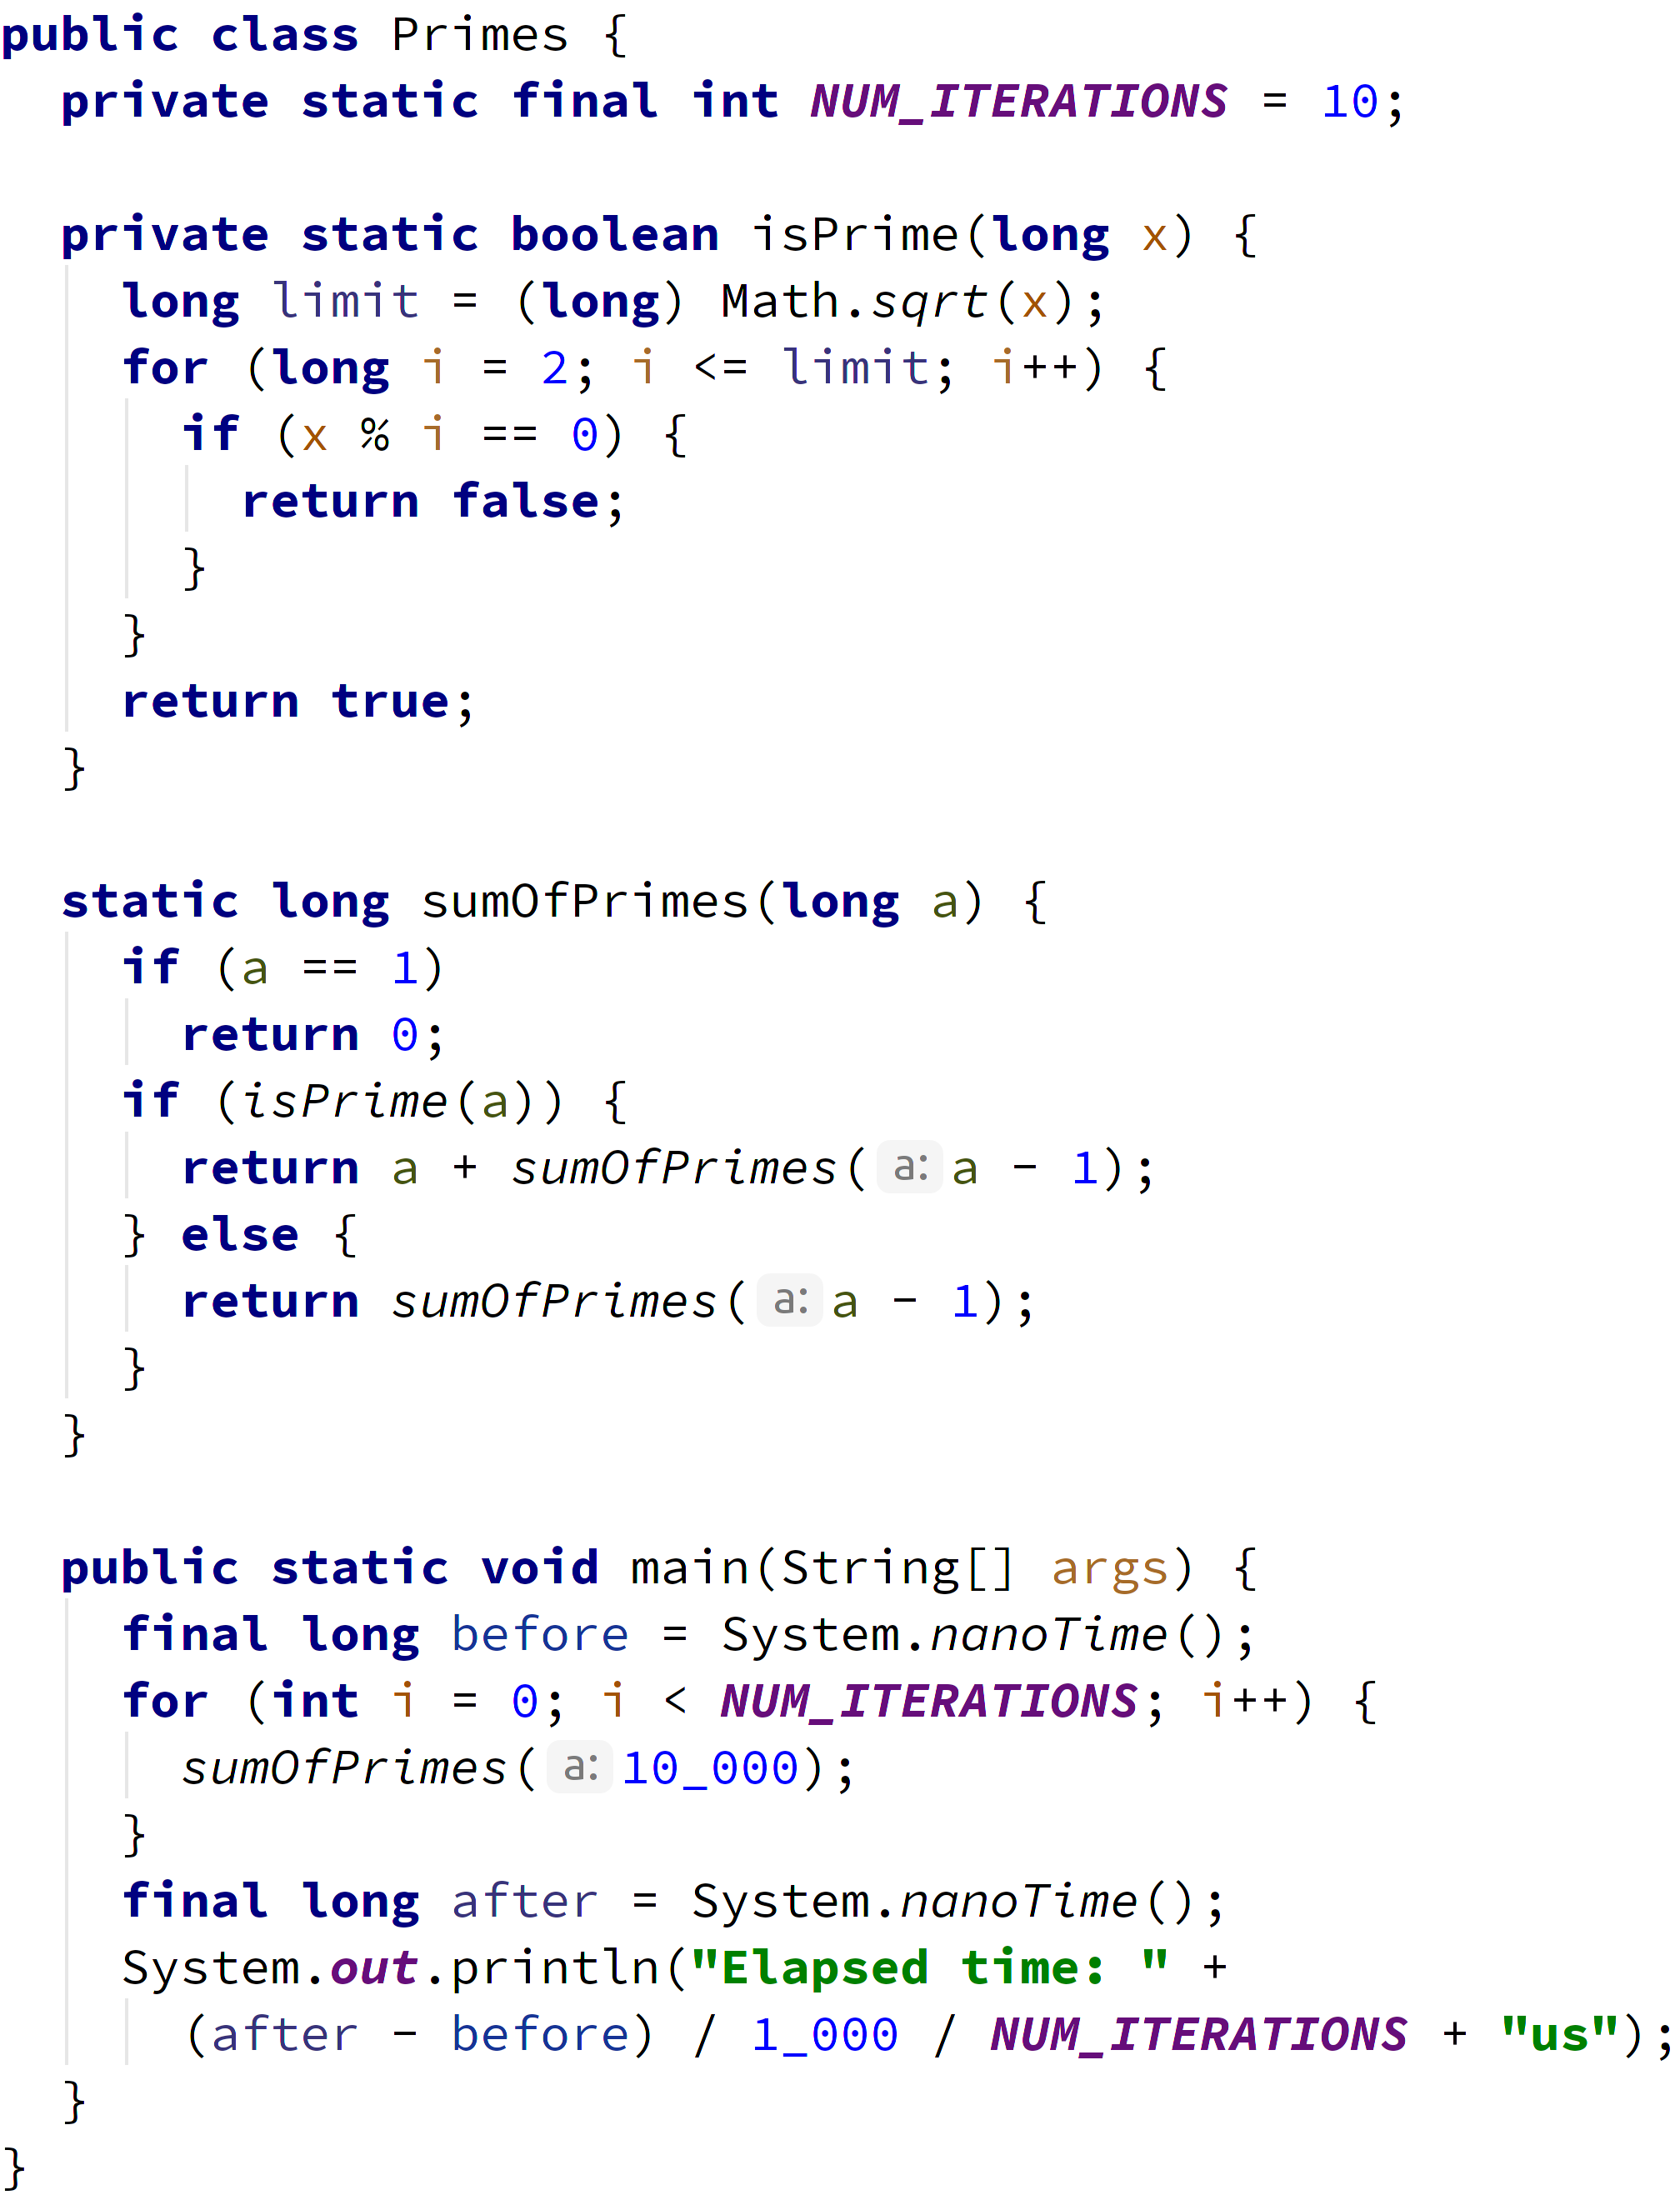
\includegraphics[height=4in]{src/img/primes-before-33.png}
        \caption{Before}
    \end{subfigure}%
    \begin{subfigure}[b]{.6\textwidth}
        \centering
        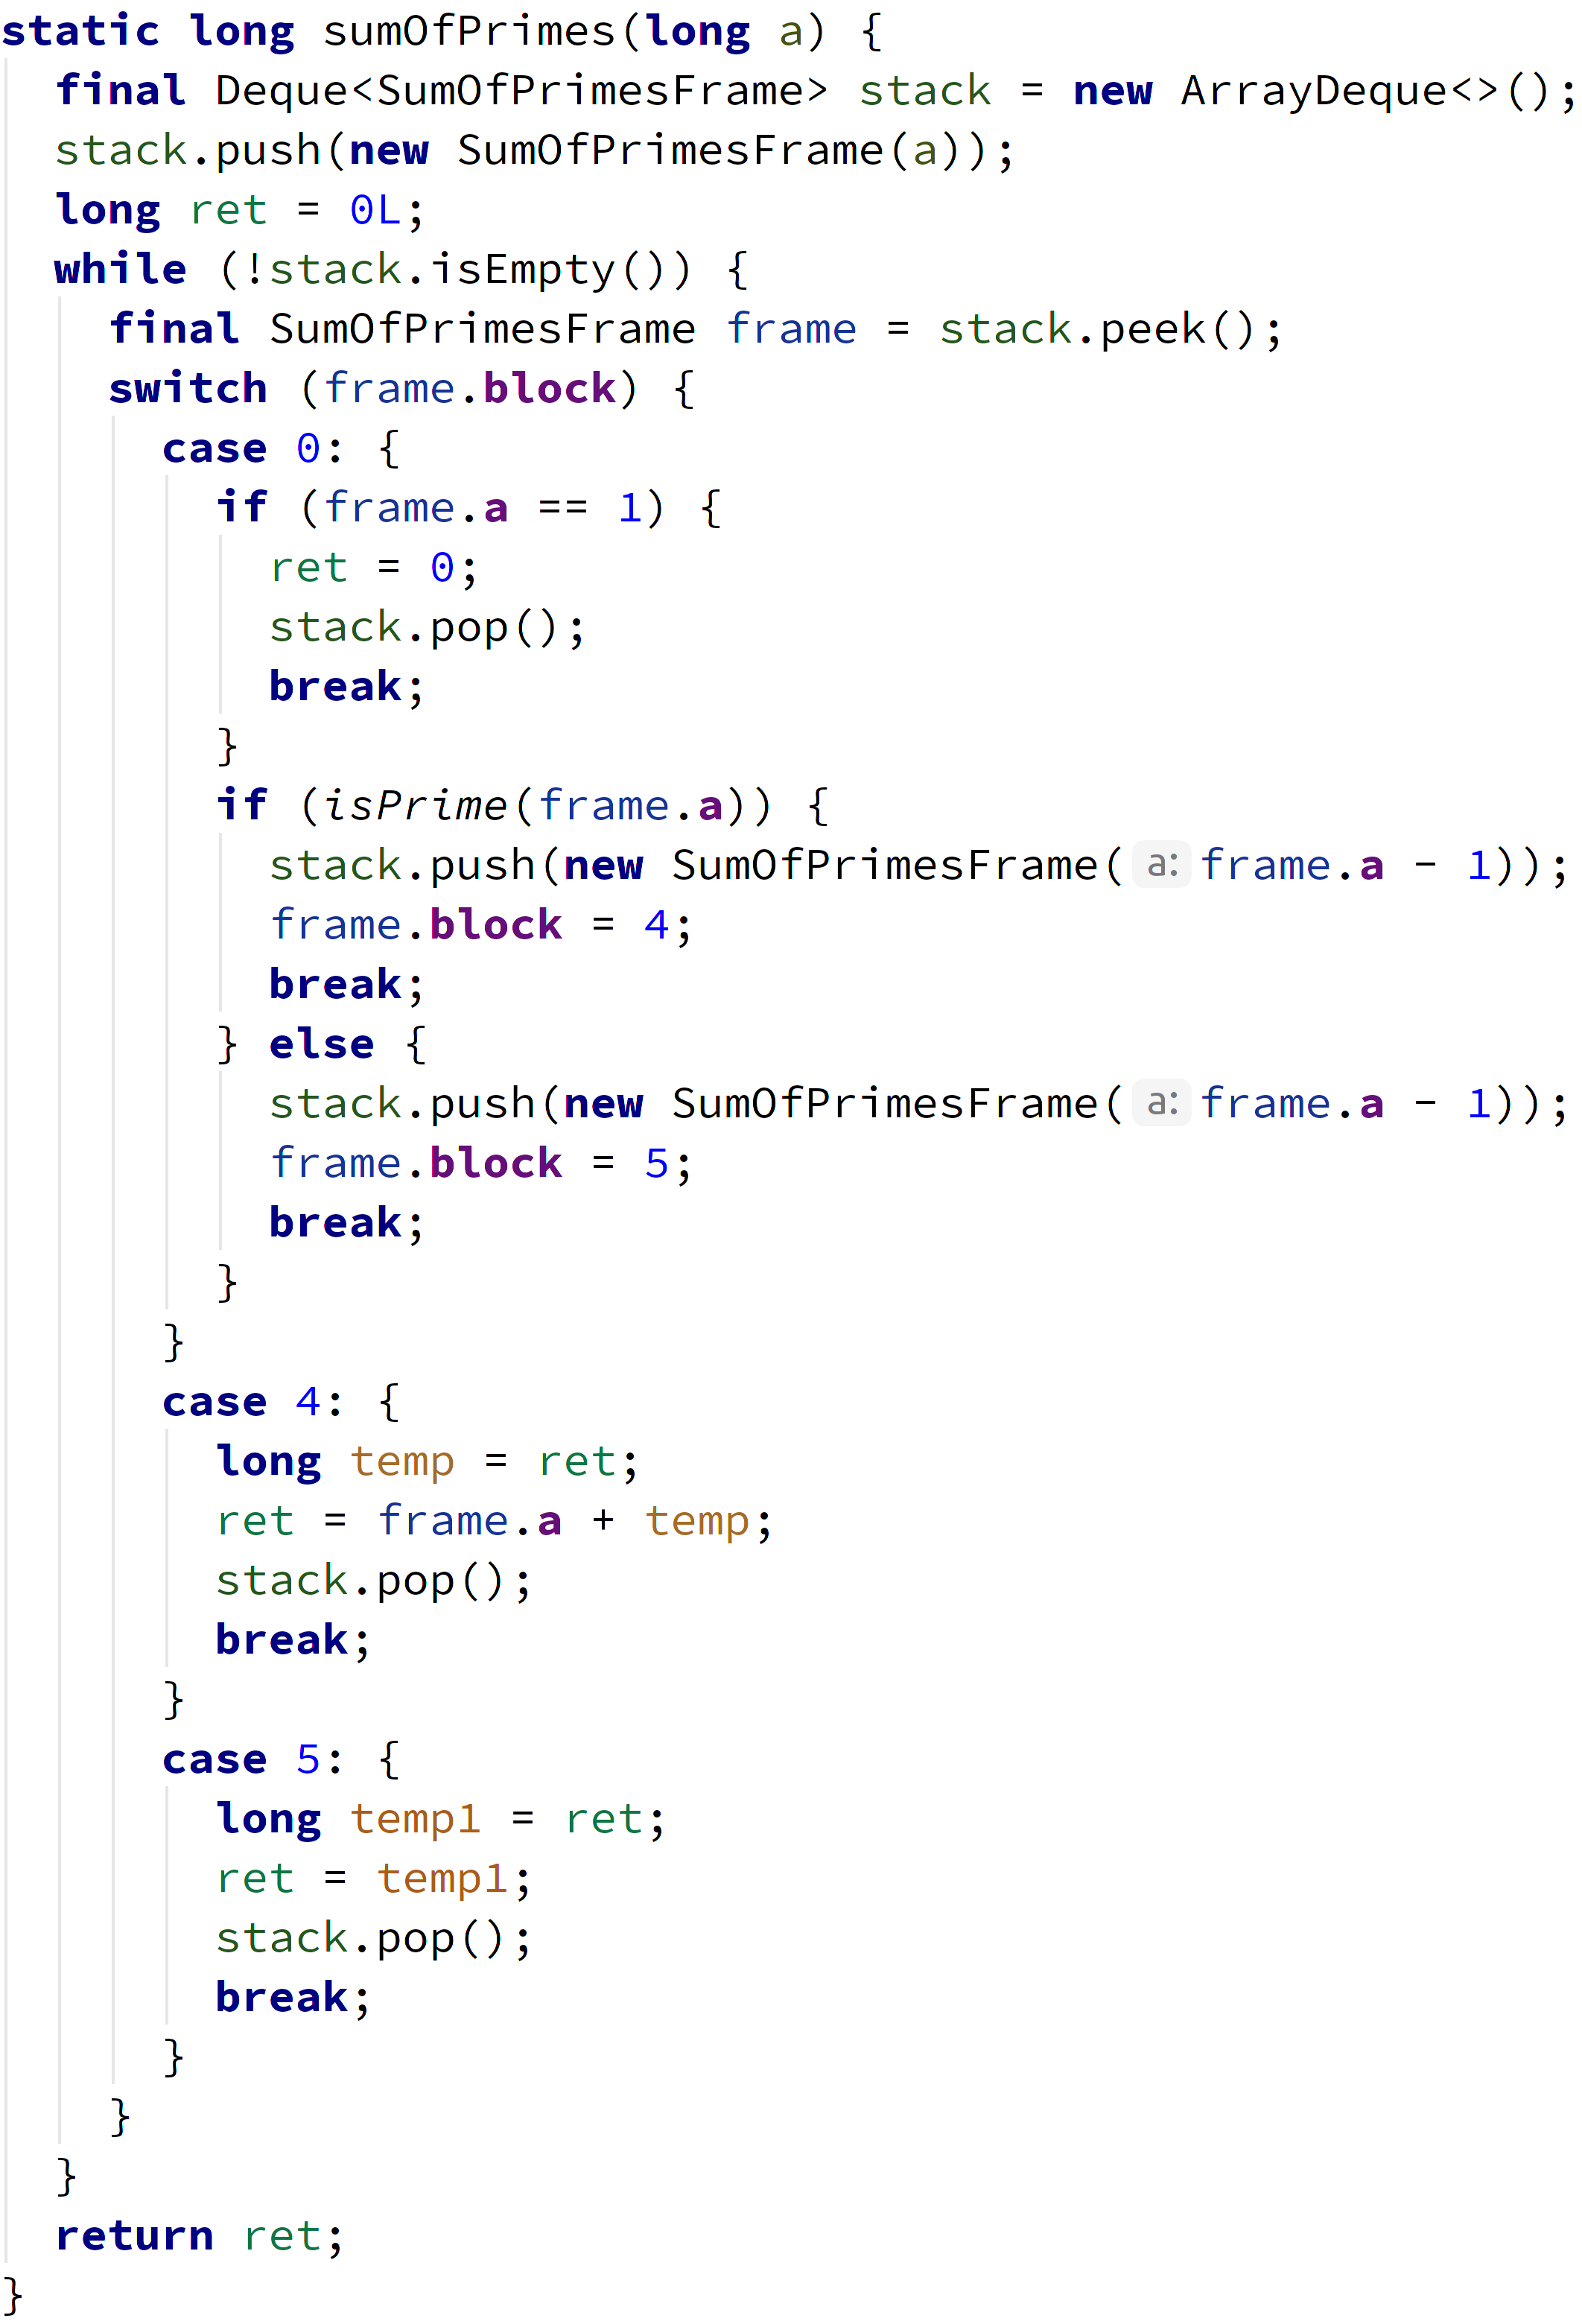
\includegraphics[height=4.72in]{src/img/primes-after-39.png}
        \caption{After}
    \end{subfigure}%
    }\\
    \caption{Computing the sum of primes smaller than a given number \label{img:primes}}
\end{figure}

The average execution time of the \code{sumOfPrimes} recursive method (measured as a mean of ten consecutive executions)
before the refactoring is \code{2444us}. The same execution time after applying the refactoring is \code{6026us}.

So the performance of the refactored method is generally worse than that of the original one. There are many
reasons why this is the case. One of them is the fact that the code of the method is split across blocks inside a
\code{switch} statement contained in a \code{while} loop, so there are more jumps through code during the execution than
in the original method. This happens because given the lack of the \code{goto} statement in Java, a workaround which
simulates it has been used.

Another performance penalty may come from the fact that after the refactoring, all the local variables in the method
body are now part of the \code{frame} object, so there is an additional overhead associated with creating these objects
and also with each access to a field of this object, which is not as fast as the access to a local variable on the stack
in the original method.

There is also an additional performance penalty associated with the \code{stack} object in the refactored method, which
uses an array-based implementation of a stack. Its capacity doubles when it gets full and the elements in the original
stack need to be copied to the array of the expanded stack when this happens.

The code of the refactored method is generally more complex than the original code of the method, so it is expected to
also be less efficient. However, there is a gain when the original method raises \code{StackOverflowError}s, because the
refactored code resolves this problem. For the example program above, when the number under whose value the sum of
primes is computed gets bigger than about \code{10000}, the original method raises a \code{StackOverflowError}. In the
case this number is equal to \code{2000000}, as in the original problem, the execution time of the refactored method is
about \code{2} seconds. It may seem much, but given the result cannot be compared to the original method, it is better
than nothing.

This refactoring should be used only when a temporary solution to \code{StackOverflowError}s is needed, as it will not
generate better code than the original one. When performance is critical, a redesign of the original algorithm to avoid
recursion is still needed.